\section{Funktionsumfang der Beispiel-Anwendung}
Damit die abgebildete Anwendung ein gutes Beispiel für eine Applikationsentwicklung darstellt, wurde beim Entwurf des Funktionsumfangs darauf geachtet, möglichst viele der typischen Funktionalitäten von Applikationen abzudecken. Eine Befragung \cite{JetBrains_miscellaneous_2021} mobiler Anwendungsentwickler durch JetBrains ergab, dass die wichtigsten Funktionen Datenspeicherung, Kommunikation über Netzwerk, Medienanzeige, Statusmanagement, Navigation, Datensynchronisierung, Dateien lesen/schreiben sind.
Das in der Arbeit betrachtete Projekt beschränkt sich dabei auf folgende Funktionalitäten:

Es soll eine App gebaut werden, die sich an der bestehende Web-Anwendung orientiert und einen Teil der Funktionalität durch die Programmierung abbildet. Dabei können die Implementierungen in zwei Gruppen unterteilt werden, die im Folgenden genauer beschrieben werden.

\subsubsection{Funktionalität mit Applikationscode}
Bei der nativen und der cross-kompilierten Applikation wird die komplette Funktionalität innerhalb der implementierten Applikation abgebildet. Die Verbindungen zwischen den umgesetzten Benutzeroberflächen ist in Abbildung \ref{fig:pageflow} dargestellt. Dabei sind Pfeile mit flacher Spitze Weiterleitungen die automatisch passieren und Pfeile ohne eine Beschriftung Abläufe, die durch das Drücken eines Buttons implementiert sind. Außerdem entsprechen die Zustände in der Abbildung den einzelnen Seiten der Anwendung. Diese sind eine Start-, Login-, Profil-, Kommunikations- und eine Chatseite. Dadurch können die oben genannte Aspekte vollständig abgedeckt werden. So ist etwa durch den Login das Statusmanagment und die Kommunikation über ein Netzwerk implementiert. 

\begin{figure}[ht]
  \centering
  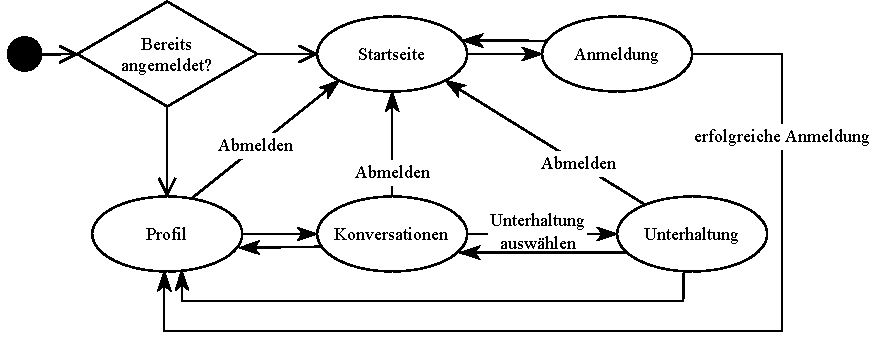
\includegraphics[height=7cm,keepaspectratio]{images/Pageflow_native_flutter.drawio.pdf} 
  \caption[Seitenablauf der implemierten nativen und cross-kompilierten Applikation]{Verbindungen zwischen den Seiten der implementierten Applikation des nativen und des cross-kompilierten Ansatzes}
  \label{fig:pageflow}
\end{figure}

Der Nutzer verwendet die Anwendung, wie im Folgenden beschrieben. Zunächst wird die App geöffnet. Wenn der Nutzer nicht eingeloggt ist, landet er auf einer Startseite/Willkommensseite, von welcher aus er sich einloggen kann. Ist er jedoch angemeldet, so wird er automatisch auf die Profil Seite weitergeleitet, auf der von einem Server geladene Daten angezeigt werden. Er kann außerdem auf das integrierte Chatsystem zugreifen und auch neue Nachrichten an andere Nutzer verschicken. Von allen Seiten mit benötigter Authentifizierung, gelangt der Nutzer durch Abmelden wieder auf die Startseite.

\subsubsection{Funktionalität mit Web-Integrierung}
In dieser Gruppe wird ein Teil oder auch die komplette Applikationslogik durch das Einbinden der Web-Anwendung in die Applikation ersetzt. So wird bei der Implementierung des hybriden Ansatzes die bereits existierende Website in eine native programmierte Applikation eingebunden. Der Applikationscode übernimmt dabei die Aufgaben, die klassischer Weise durch ein Framework erfüllt werden würde. Sie ist jedoch durch die spezifische Implementierung der Webseite stark in der Funktionalität eingeschränkt.

Bei der gemischten   Implementierung wird zwischen der Web-Anwendung und Benutzeroberflächen, die mit dem Cross-Compiler Framework Flutter erstellt wurden, gewechselt. Dabei werden insbesondere der Login, die Profilseite und das Chat System durch Flutter Seiten ersetzt, während der Rest der Anwendung durch die Web-Anwendung dargestellt wird. Daher ist dieser Ansatz eine Mischung aus dem hybriden und dem cross-kompilierten Ansatz.


